\subsection{Experimental animals}

We used three transgenetic zebrafish from Janelia farm with a good expression of Gcamp6 gen ($tg(HuC:GCamp6f)jf7$). For the experiments, the zebrafish were 5-6 days postfertilization (dpf) old. In two of the three, we recorded behavioral data.    

\subsection{Experimental setup}

The stimulation arena consisted of a glass bulb that was coated in paint to be able to project light on it from the outside. The light was produced by a high power LED light source (CHROLIS-C1, Thorlabs Incorporated) and transmitted to a projector (DLP® LightCrafter™ 4500, Texas Instruments Incorporated) using a liquid light guide. The light exiting the projector was then reflected downwards in a \SI{90}{\degree} angle onto a square pyramidal mirror, that split the beam into four. Each of the four beams was then reflected by one of the four mirrors placed around the setup and consequently projected onto the glass sphere. The result is a spherical projection. The experimental setup is visualized in figure \ref{fig:setup}. The fish were embedded in Agarose on a custom designed stage that could be fixed inside the stimulus arena.  

\begin{figure}[H]
    \centering
    \includegraphics[width=0.6\textwidth]{figures/setup.pdf}
    \mycaption{CAD rendering of the experimental setup.}{\textbf{A} shows the whole recording setup excluding the camera recording behaviors of the fish. The fish is fixed inside a glass bulb (a) containing E3 medium. The light is produced by an LED light source (c), transferred to a projector (b) and projected onto a \SI{45}{\degree} mirror (d). The mirror reflects the projection onto a pyramid mirror (not visible in the current rendering), which splits the beam into four. The four beams are then reflected by four mirrors placed around the setup (e) and reflected onto the glass bulb from four sides. The result is a spherical projection into the glass bulb.The calcium activity was recorded by a moving objective microscope that peeks through an opening in the top of the glass sphere (g). \textbf{B} shows the camera (f) used to record through the bottom of the glass bulb using mirrors as well. Images are courtesy of Tim Hladnik.}
    \label{fig:setup}
\end{figure}

\subsubsection{Embedding procedure}

\begin{wrapfigure}{R}{0.5\textwidth}
    \vspace{-0.3cm}
    
\includegraphics[width=\linewidth]{figures/drawing.pdf}
    \mycaption{Agarose stage}{ to fixate the larvae. The stage consisted of a diagonal cut-off of a pipette tip (orange) and a small, pointed Agarose table (blue). The fish (gray) were separately embedded into a drop of Agarose. We pruned the edges and then placed the Agarose block containing the fish onto the point of the Agarose table.}
    \label{fig:stage}
\end{wrapfigure}

The immobilization of the fish was conducted with \SI{1.6}{\percent} low-melting Agarose, where it was submerged for a short time before a drop of Agarose containing the fish was placed on a Petri-dish to polymerize. Meanwhile, the plastic pipette was prepared (diagonal cut-off, see figure \ref{fig:stage}), placed on a 3D-printed stage, and filled with \SI{2}{\percent} Agarose. After \SI{30}{\minute} the stage was separated from the now polymerized Agarose. The immobilized fish was placed on the tip of the Agarose that stood out from the pipette tip. To combine the Agarose from the pipette and the Agarose where the fish was in, we added \SI{1.6}{\percent} Agarose which filled the gap between those two Agarose blocks. The pipette was then inserted into a holding apparatus inside the glass sphere, which we filled with E3. For two of the three fish, we removed the Agarose around the eyes of the fish, so that the fish can move them (Figure \ref{fig:stage}). 

\subsubsection{Stimulus}

The stimulus consisted of red and green gratings with six different logarithmically increasing contrast levels (0., 0.1, 0.18, 0.32, 0.56, 1.0) that were randomized. The stimulus time for one contrast level was 8 seconds long, divided into 4 seconds of no angular velocity and followed by 4 seconds with an angular velocity of \SI{30}{\degree\per\second}. Two directions of velocity were used and they were randomized. This protocol was repeated 3 times and the order stayed the same across the repeats. Before the protocol started and after the protocol ended we implemented a pause with no stimulus for 15 seconds. The stimulus was generated using \href{https://github.com/thladnik/vxPy}{vxPY} (\href{https://github.com/thladnik/vxPy}{https://github.com/thladnik/vxPy}). The color contrast levels of the stimulus we displayed for this experiment were not yet linearised and which contrast levels the fish exactly perceived are unknown. 

\subsubsection{Calcium imaging}

Calcium imaging was conducted with an infrared laser (Coherent Vision-S Ti-Sa laser, and a 25 x objective (Nikon CFI75, Tokyo, Japan),  a wavelength of \SI{920}{\nano\meter}), with a movable objective microscope (MOM) (Sutter Instruments, Novato, CA, USA). The resolution of the calcium imaging was \SI{2}{\hertz}. Before beginning the imaging protocol we checked if the fish was drifting out of the focal plane. For this procedure, we took a reference image and waited for \SI{30}{\minute}, after that time we retook the image, compared it with our reference image and decided to start our stimulus protocol or to wait another \SI{30}{\minute}. Calcium imaging was done in \SI{10}{\micro\meter} intervals along the optical axis. After each recording, we visually assessed the drift of the Agarose. If drifting occurred, we did not consider these recordings for the data analysis. For our three fish, we used 12, 5, and 5 recordings. For processing the Calcium-imaging data, we used suite2p, an open-source pipeline for processing two-photon calcium imaging data \parencite{Pachitariu061507}.

\subsubsection{Behavioral response}

For a behavioral measure of the sensitivity to isoluminant chromatic motion stimuli, we chose the optokinetic response (OKR). 
Eye movements were recorded via a camera that recorded the bottom of the larva through a \SI{45}{\degree} mirror below the glass bulb (see figure \ref{fig:setup}). A small area on the bottom of the bulb was not coated in paint and thus enabled a clear view into the underside of the fish. Image segmentation and eye tracking happened in real-time using \href{https://github.com/thladnik/vxPy}{vxPY} (\href{https://github.com/thladnik/vxPy}{https://github.com/thladnik/vxPy}). Eye velocities were recorded in degrees per second at a rate of \SI{20}{\hertz}.  

\subsection{Data analysis}

We wrote our data analysis pipeline in Python 3.10.9 using the packages Numpy \parencite{harris2020array}, Scipy \parencite{2020SciPy-NMeth}, Matplotlib \parencite{Hunter:2007}, vxPy (\href{https://github.com/thladnik/vxPy}{https://github.com/thladnik/vxPy}) and suite2p \parencite{Pachitariu061507}. All scrips used for the analysis and plotting are publically available in a \href{https://github.com/weygoldt/colorblind-directioncells}{git repository}.

\subsubsection{Calcium data}

First, we computed the $\operatorname{dff}$ of the fluorescence signal of every single ROI by formula \ref{eq:dff}.

\begin{equation}
    \operatorname{dff}(t) = \frac{f_{ROI}(t) - \langle f_{ROI}(t) \rangle}{\langle f_{ROI}(t) \rangle}
    \label{eq:dff}
\end{equation}

Where the difference between the fluorescence of a single point in time $f_{ROI}(t)$ and the mean of the signal over time is divided by the mean. We further used the $\operatorname{dff}$ to compute the Z-score to quantify calcium activity (equation \ref{eq:zscore}).

\begin{equation}
    Z = \frac{\operatorname{dff}(t) - \langle \operatorname{dff}(t) \rangle}{\sigma_{\operatorname{dff}(t)}}
    \label{eq:zscore}
\end{equation}

The Z-score indicates how many standard deviations a certain point in time deviates from the mean of the signal, in this case, the $\operatorname{dff}$ of the signal. This is particularly useful in this context because peaks that originate from noise (in signals with a large standard deviation) are scaled down relative to peaks with a good signal-to-noise ratio. To simplify the analysis of multiple time series with different sampling rates, we computed for every separate stimulation phase the mean of the z-score and dff. This was possible because the sampling rate of the microscope was relatively low (\SI{2}{\hertz}) and the stimulation phases were short. Taking the means significantly simplified the analysis while resulting in a minor loss of temporal resolution.

\vspace{\baselineskip}

\begin{figure}[ht]
    \centering
    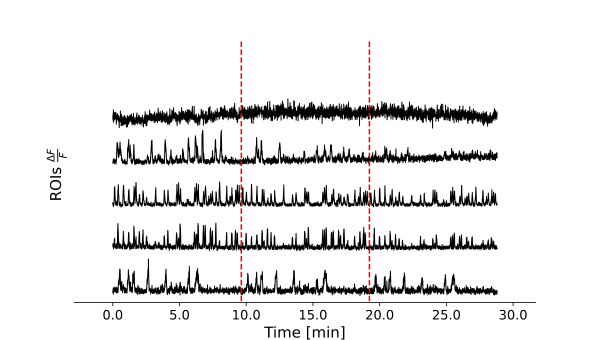
\includegraphics[width=0.8\linewidth]{figures/autocorrelation.pdf}
    \mycaption{Calcium signal (Z-score) over time }{ from various ROIs. Red lines indicate the three repetitions.}
    \label{fig:autocorrelation}
\end{figure}

Since we targeted specifically direction selective cells, we constructed a data filtering pipeline that only provides the ROIs that respond to movements in a certain direction. In a first filtering step we excluded all individuals that did not respond to the stimulus. To do so, we computed the Spearman correlations between the z-scores of the same ROI across the three identical repeats of the stimulation. This resulted in three correlation coefficients per ROI, from which we then took the mean. To choose the units with the strongest auto-correlation, we estimated the distribution of the resulting correlation coefficients by a convolution with a Gaussian kernel. We then chose the ROIs that fell into a 20\% integral of the right tail of the distribution (Figure \ref{fig:autocorrelation}).

\begin{figure}[H]
    \centering
    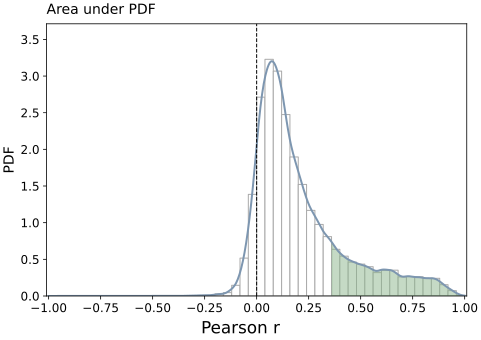
\includegraphics[width=0.8\linewidth]{figures/pcorrelation.pdf}
    \mycaption{Probability density of autocorrelations.}{ \textbf{Left:} Probability density function of the mean correlation coefficients computed between the stimulation repeats of a single ROI. The green tail indicates the area that was chosen to include the 'active' ROIs, i.e. the ones that were correlated strongly between the trials, which indicates repeatable response to the stimulus. \textbf{Right: }Difference gradient that was used to obtain all ROIs that fall into the green area. To obtain this, we computed the area under the curve (AUC) between the one and an array of index values and then subtracted it from our target AUC of 0.2.}
    \label{fig:pcorrelation}
\end{figure}

In a next filtering step, we had to select all ROIs that responded specifically to either clockwise or counterclockwise motion. To do so, we created motion regressors for either direction and correlated them with the z-scores. All ROIs that crossed the correlation threshold of 0.2 were included in the analysis. Figure \ref{fig:regressor} shows an example of some z-scores and the regressors. In a next step, we removed all stimulus phases where no motion stimulus was presented and then computed the means and standard deviations for each stimulus categories for all fish and all repeats for a single fish. 

\begin{figure}[H]
    \centering
    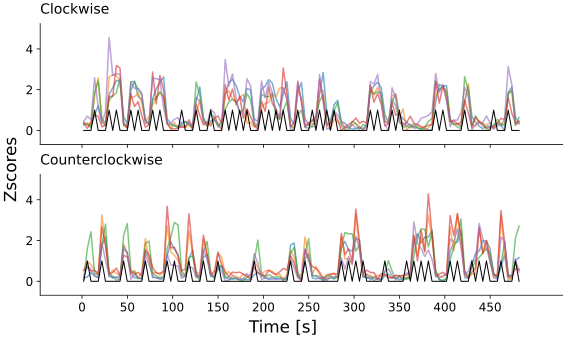
\includegraphics[width=0.8\linewidth]{figures/regressor.pdf}
    \mycaption{Motion-direction regressors and correlated z-scores. }{The black line show the regressors for clockwise (cw, top) and counterclockwise (ccw, bottom) respectively. The gray lines indicate the z-scores of some ROIs that were strongly correlated with the respective regressors.}
    \label{fig:regressor}
\end{figure}

\subsubsection{Behavioral data}

As a behavioral measure we chose the eye velocities. To make the velocities comparable across the stimulus categories we removed saccades in the signal by a median filter with a width of 41 data points. As in the calcium signal, we then computed the mean eye velocity for each stimulus phase. The second step of abstraction was to compute the means and standard deviations across stimulus repeats and across the two individuals we recorded behavioral data for.  

\FloatBarrier